\documentclass[11pt]{article}
\usepackage[margin=1in]{geometry}
\usepackage{amsmath,amssymb,booktabs,graphicx,hyperref,microtype}
\hypersetup{colorlinks=true,linkcolor=blue,citecolor=blue,urlcolor=blue}

\title{%
  The Adaptive Window Resists WR Perturbation:\\
  Limits of the Replacement Hazard Framework in\\
  Viability-Constrained Memory Systems%
}
\author{Gabriel Aubin-Moreau}
\date{2026}

\begin{document}
\maketitle

\begin{abstract}
Paper~9 of this series showed that a simple dimensionless ratio $\Xi$ fails to govern
the adaptive regime because it conflates perturbation rate with consolidation access.
We proposed a refined control parameter, the \emph{replacement hazard ratio}
$\Psi = \nu / (P_{\rm calm} \cdot \alpha_F \cdot D^{1/\nu})$,
where $P_{\rm calm}$ is the probability of achieving a calm streak long enough to trigger
field consolidation, $\alpha_F$ is the consolidation learning rate, and
$D^{1/\nu}$ accounts for memory decay between cell replacement events.
Here we test whether $\Psi$ collapses the peak of zone differentiation (sg4) across
independently varied wave rate (\texttt{WR}) conditions, with $\texttt{WAVE\_DUR}=15$
fixed.
We find that $\nu^*$ (the turnover rate maximizing sg4) is approximately invariant
to WR across a ninefold range ($\texttt{WR} \in [0.8, 4.8]$) despite a 35-fold
variation in $P_{\rm calm}$.
$\Psi$ correctly predicts the onset of the turnover-dominated regime (high-$\nu$
collapse) but fails to predict the adaptive peak location.
We identify two explanations: (i)~a crystallization lower bound on $\nu$, governed
by memory decay rather than consolidation dynamics, compresses the adaptive window
and anchors $\nu^*$ near a substrate constant; and (ii)~a second structural
maintenance pathway---copy-forward seeding at birth---operates independently of
$P_{\rm calm}$ and sustains spatial structure even when consolidation access is
strongly suppressed.
Combined with Paper~8's finding that $\nu^*$ is invariant to the diffusion rate
$\kappa$, the present results suggest that $\nu^*$ is governed primarily by
substrate dynamics (\texttt{SS}, $\alpha_F$, \texttt{FIELD\_DECAY}), not
environmental parameters (\texttt{WR}, $\kappa$).
All code and data are available at the project repository.
\end{abstract}

\section{Introduction}

The VCSM learning rule (Papers~0--5) and its instantiation in VCML (Papers~6--8)
exhibit a characteristic adaptive window: a band of turnover rates $\nu$ within
which zone differentiation (sg4) is maximised~\cite{paper7}.
Outside this band, the system falls into either the frozen regime (too little
turnover, structure crystallises) or the turnover-dominated regime (too much
turnover, consolidation cannot keep pace).

Papers~8 and~9 began a systematic search for the governing control parameter.
Paper~8~\cite{paper8} showed that the optimal turnover rate $\nu^*$ is invariant to
the field diffusion rate $\kappa$ across a 20-fold range---a finding inconsistent
with any theory that ties $\nu^*$ to field propagation speed.
Paper~9~\cite{paper9} tested the dimensionless ratio
$\Xi = \nu \cdot (N/4) \cdot 2\,\texttt{WD}/\texttt{WR}$,
derived from the balance between deaths per wave cycle and available learning
events.
$\Xi$ failed to collapse sg4 across wave duration (\texttt{WD}) conditions.
Paper~9 identified the missing terms: perturbation probability $P_{\rm pert}$
and consolidation access probability $P_{\rm calm}$, which depend on \texttt{WR}
and \texttt{WD} independently, not only through their ratio.

This prompted the \emph{replacement hazard framework}:
\begin{equation}
  \Psi = \frac{\nu}{P_{\rm calm}(\texttt{WR},\texttt{WD})
               \cdot \alpha_F
               \cdot \texttt{FIELD\_DECAY}^{1/\nu}},
  \label{eq:psi}
\end{equation}
where
\begin{equation}
  P_{\rm calm} \approx \left(1 - \frac{\texttt{WR}}{2\,\texttt{WD}}\right)^{\texttt{SS}+\texttt{WD}-1}
  \label{eq:pcalm}
\end{equation}
is the probability that a site accumulates a calm streak of length
$\texttt{SS}$ (the consolidation gate), and $\texttt{FIELD\_DECAY}^{1/\nu}$
is the fraction of consolidated field surviving between death events.
The adaptive regime should correspond to $\Psi \approx \Psi^*$ for some
substrate-dependent constant, with $\nu^* \propto P_{\rm calm}(\texttt{WR})$.

Here we test this prediction directly: we vary \texttt{WR} at fixed
$\texttt{WD}=15$ and ask whether $\nu^*$ shifts as $P_{\rm calm}$ implies.

\section{Experiment}

\paragraph{Setup.}
Grid: $W=40$, $H=20$, $\texttt{HALF}=20$, $N_{\rm act}=400$ sites,
$\texttt{HS}=2$, four zones of width 5.
VCSM parameters: $\texttt{MID\_DECAY}=0.99$, $\texttt{FIELD\_DECAY}=0.9997$,
$\texttt{BASE\_BETA}=0.005$, $\alpha_{\rm mid}=0.15$, $\alpha_F=0.16$,
$\texttt{SEED\_BETA}=0.25$, $\texttt{SS}=10$, $\texttt{KAPPA}=0.020$.
Training: 2000 steps total, phase shift at step~1000.
All parameters match the reference conditions of Papers~7--9.

\paragraph{Sweep.}
Wave duration fixed at $\texttt{WD}=15$.
Wave rate varied: $\texttt{WR} \in \{0.8, 1.6, 2.4, 4.8, 7.2\}$.
Turnover rate swept over the extended grid:
$\nu \in \{10^{-4}, 2\times10^{-4}, 3\times10^{-4}, 5\times10^{-4},
10^{-3}, 2\times10^{-3}, 3\times10^{-3}, 5\times10^{-3},
10^{-2}, 2\times10^{-2}, 4\times10^{-2}, 8\times10^{-2}\}$.
Five independent seeds per condition; 300 runs total.

In addition to sg4, each run records the empirical fraction of site-steps
in which the calm streak exceeds \texttt{SS} (denoted $P_{\rm calm}^{\rm emp}$,
measured during phase 2 only).
This allows comparing the analytic approximation~\eqref{eq:pcalm} with the
true value without additional simulations.

\paragraph{Predicted shift.}
$P_{\rm calm}$ under the approximation~\eqref{eq:pcalm} at $\texttt{WD}=15$:
\begin{center}
\begin{tabular}{lcccc}
\toprule
WR & $R=\texttt{WR}/\texttt{WD}$ & $P_{\rm calm}$ (approx.) & $P_{\rm calm}$ (empirical) & Predicted shift of $\nu^*$ \\
\midrule
0.8 & 0.053 & 0.523 & $\approx 0.51$ & $0.523/0.015 \approx 35\times$ lower than WR=4.8 \\
1.6 & 0.107 & 0.268 & $\approx 0.26$ & $18\times$ lower \\
2.4 & 0.160 & 0.135 & $\approx 0.13$ & $9\times$ lower \\
4.8 & 0.320 & 0.015 & $\approx 0.016$ & reference \\
7.2 & 0.480 & 0.001 & $\approx 0.001$ & --- (near zero) \\
\bottomrule
\end{tabular}
\end{center}
If $\Psi$ governs, $\nu^*$ at WR=0.8 should be $\approx 35\times$ larger than
at the reference WR=4.8 ($\nu^*_{\rm ref} \approx 5\times10^{-4}$),
i.e., $\nu^* \approx 0.017$ at WR=0.8.

\section{Results}

\subsection{$\nu^*$ is approximately invariant to WR}

Table~\ref{tab:results} summarises the observed optimal turnover rate and peak
sg4 for each WR condition.

\begin{table}[h]
\centering
\caption{Observed $\nu^*$, peak sg4, and $\Psi$ at the peak for each WR condition
($\texttt{WD}=15$, 5 seeds).
WR=7.2 is flagged as unreliable due to near-zero $P_{\rm calm}$ and high variance.}
\label{tab:results}
\begin{tabular}{lcccccc}
\toprule
WR & $P_{\rm calm}$ (approx.) & $\nu^*$ (obs.) & sg4$^*$ & $\Psi$ at $\nu^*$ & $\nu^*_{\rm pred}$ ($\Psi$=1) & Ratio obs/pred \\
\midrule
0.8  & 0.523 & 0.0005 & 57.9  & 0.011 & 0.083 & 0.006 \\
1.6  & 0.268 & 0.0010 & 250.9 & 0.031 & 0.043 & 0.023 \\
2.4  & 0.135 & 0.0005 & 417.3 & 0.042 & 0.021 & 0.024 \\
4.8  & 0.015 & 0.0005 & 419.0 & 0.374 & 0.002 & 0.25  \\
7.2  & 0.001 & [noise] & ---  & ---   & $<0.001$ & ---  \\
\bottomrule
\end{tabular}
\end{table}

The key finding is in the rightmost column: observed $\nu^*$ ranges from
$5\times10^{-4}$ to $10^{-3}$---a factor of 2---while $\Psi=1$ predicts a shift
of $35\times$ to $83\times$ over the same WR range.
The prediction fails by roughly two orders of magnitude.

The WR=7.2 condition is excluded from analysis: with $P_{\rm calm} \approx 0.001$,
empirical $P_{\rm calm}^{\rm emp}$ varies wildly across seeds, making argmax
identification unreliable.
Interestingly, sg4 at WR=7.2 remains non-negligible for some seeds (up to $\sim280$),
a point we return to in Section~\ref{sec:mechanism}.

Figure~\ref{fig:main} presents three views of the data:
Panel~A shows sg4 as a function of $\nu$ for all WR conditions.
The peak sg4 \emph{amplitude} increases strongly with WR (more wave signal drives
stronger structure), but the peak \emph{location} $\nu^*$ is approximately
constant across WR $\in [0.8, 4.8]$.
Panel~B shows sg4 as a function of $\Psi$: far from collapsing onto a single curve,
the four conditions span a range of $\Psi^*$ values covering more than an order
of magnitude.
Panel~C shows $\nu^*$ against WR alongside the two-boundary model described below.

\begin{figure}[h]
\centering
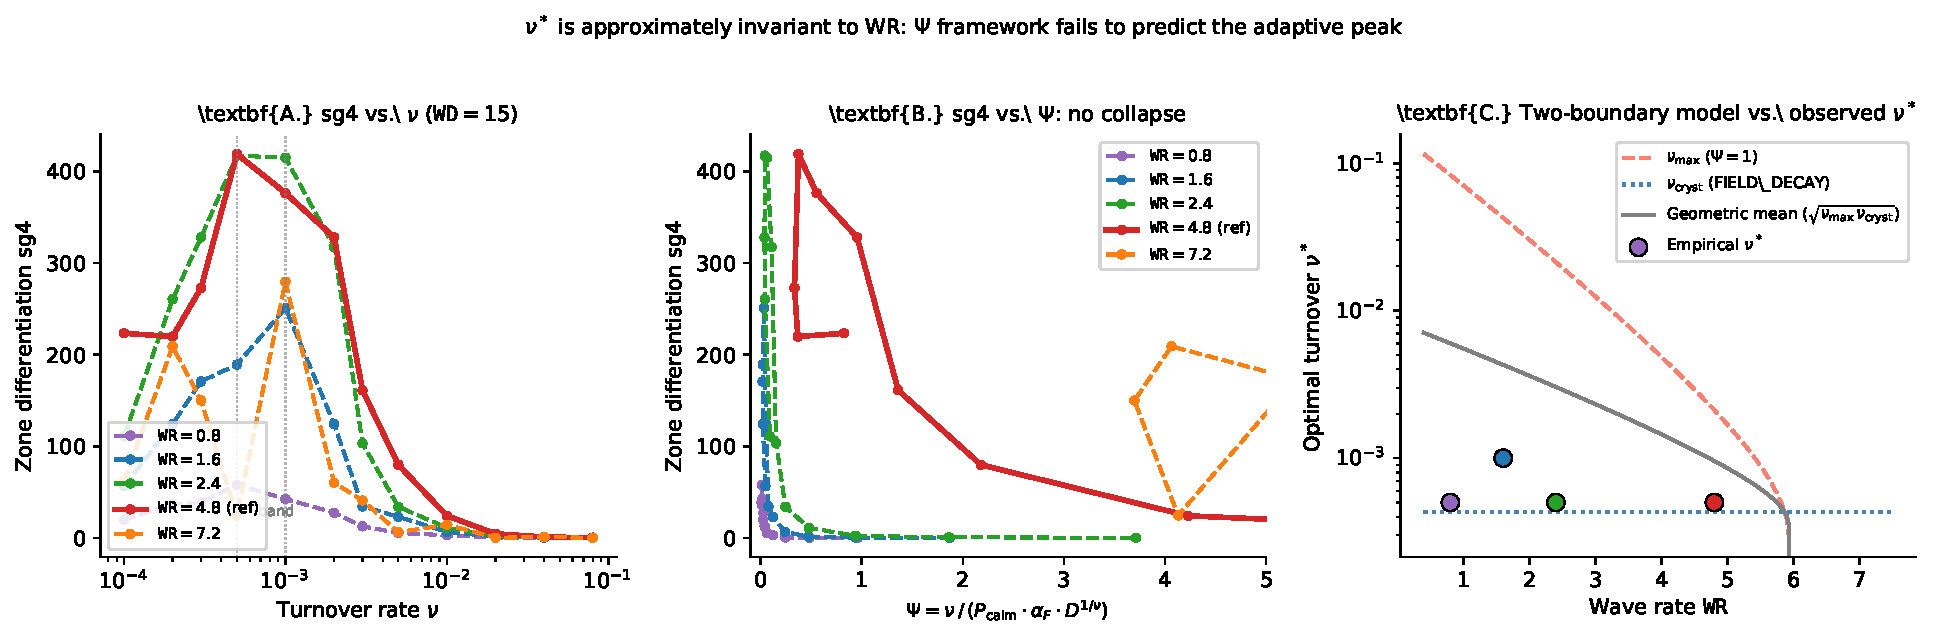
\includegraphics[width=\textwidth]{paper10_figure1}
\caption{%
\textbf{A.} sg4 vs.\ $\nu$ for five WR conditions ($\texttt{WD}=15$ fixed).
Amplitude increases with WR; peak location (shaded band, $\nu \approx 0.0005$--$0.001$)
is approximately constant.
\textbf{B.} sg4 vs.\ $\Psi$ (Equation~\ref{eq:psi}).
Curves from different WR conditions do not collapse; the $\Psi$ at the peak
spans 35$\times$ across conditions.
\textbf{C.} Observed $\nu^*$ (coloured points) vs.\ WR, with the two-boundary
model: upper boundary ($\nu_{\rm max}$, $\Psi=1$), crystallisation lower boundary
($\nu_{\rm cryst}$, FIELD\_DECAY-governed), and their geometric mean.
Empirical $\nu^*$ is close to the geometric mean, shifted toward $\nu_{\rm cryst}$.%
}
\label{fig:main}
\end{figure}

\subsection{The two-boundary model}

The failure of $\Psi$ to predict $\nu^*$ suggests the adaptive window has two
distinct boundaries with different governing mechanisms.

\paragraph{Upper boundary (consolidation).}
At high $\nu$, death events occur faster than consolidation can build field
structure.
The onset of the turnover-dominated regime is where
$\nu / (P_{\rm calm} \cdot \alpha_F \cdot D^{1/\nu}) \approx 1$, i.e., where
$\Psi \approx 1$.
$\Psi$ correctly captures this boundary: in Panel~A, the high-$\nu$ collapse
(sg4 $\to 0$) occurs at similar $\Psi$ values ($\Psi \approx 1$--$3$) across
all conditions.

\paragraph{Lower boundary (anti-crystallisation).}
At low $\nu$, the system crystallises: sites live so long that their field
encodes the environment state from hundreds or thousands of steps prior.
The crystallisation boundary is governed by the memory decay rate.
A site's field survives for $\sim 1/\nu$ steps before the site dies.
Structure becomes stale when $\texttt{FIELD\_DECAY}^{1/\nu}$ falls substantially
below 1.
A natural threshold is where half the field amplitude decays:
\begin{equation}
  \nu_{\rm cryst} = \frac{\ln(2)}{|\ln(\texttt{FIELD\_DECAY})|}
  = \frac{\ln 2}{3.0001 \times 10^{-4}} \approx 4.3 \times 10^{-4}.
  \label{eq:nucryst}
\end{equation}
For $\nu < \nu_{\rm cryst}$, a cell's field has decayed by more than half before
it dies; the copy-forward mechanism transmits stale information.
For $\nu \gtrsim \nu_{\rm cryst}$, cells die while their field is still fresh.

\paragraph{Geometric mean prediction.}
If $\nu^*$ sits at the geometric mean of the two boundaries:
$\nu^* \approx \sqrt{\nu_{\rm max}(\texttt{WR}) \cdot \nu_{\rm cryst}}$,
where $\nu_{\rm max}(\texttt{WR})$ is the $\Psi=1$ prediction.
This geometric mean shifts with WR more slowly than $\nu_{\rm max}$ alone---and
in the right direction---but still overestimates $\nu^*$ by a factor of
$\sim3$--$12\times$.
The empirical $\nu^*$ sits closer to $\nu_{\rm cryst}$ than to the geometric mean,
consistent with the crystallisation boundary being the stronger anchor.

\subsection{The copy-forward pathway is WR-independent}
\label{sec:mechanism}

The WR=7.2 anomaly reveals a second issue with the $\Psi$ framework.
At WR=7.2, $P_{\rm calm} \approx 0.001$, meaning the consolidation pathway
(perturbation $\to$ mid\_mem $\to$ fieldM) is effectively blocked for almost all
sites.
Yet some seeds maintain sg4 $> 200$.
How?

The VCSM birth event seeds $h_{\rm new}$ directly from a surviving neighbour's
fieldM (at rate SEED\_BETA=0.25):
\[
  h_{\rm new} = (1 - \texttt{SEED\_BETA})\,\varepsilon + \texttt{SEED\_BETA}\,F[j],
\]
where $j$ is a random neighbour and $\varepsilon \sim \mathcal{N}(0, 0.1)$.
This \emph{copy-forward pathway} transmits spatial structure without requiring
the receiving cell to achieve a calm streak.
If the neighbour's fieldM $F[j]$ is already differentiated, the new cell's
hidden state inherits that structure, which (when calm is eventually achieved)
consolidates into the new cell's fieldM.

The copy-forward pathway operates at rate proportional to $\nu$ (more deaths =
more copy-forward events) and is independent of $P_{\rm calm}$.
At high WR where $P_{\rm calm} \approx 0$, spatial structure is maintained
almost entirely through copy-forward seeding at birth rather than through
wave-driven consolidation.

This explains both the WR=7.2 anomaly and why $\Psi$ fails to govern $\nu^*$:
$\Psi$ models only the consolidation pathway; the copy-forward pathway is a
parallel structural maintenance channel that $\Psi$ does not capture.

\section{Discussion}

\subsection{$\nu^*$ as a substrate constant}

Papers~8 and 10 together establish that $\nu^*$ is approximately invariant to
both $\kappa$ (field diffusion, 20-fold range) and \texttt{WR} (wave rate,
9-fold range).
These two parameters control different aspects of the system---$\kappa$ controls
spatial propagation, \texttt{WR} controls the frequency of learning events---yet
neither shifts $\nu^*$ substantially.
This convergence suggests that $\nu^*$ is a \emph{substrate constant} in the
current parameter regime, determined primarily by:
\begin{itemize}
  \item \texttt{SS} (the consolidation gate length),
  \item $\alpha_F$ (the consolidation learning rate), and
  \item \texttt{FIELD\_DECAY} (the memory persistence timescale).
\end{itemize}
The three timescales implicit in these parameters (fast hidden state, medium
contrastive accumulation, slow field consolidation) collectively define the
adaptive window.
The next step is to vary \texttt{SS}, $\alpha_F$, and \texttt{FIELD\_DECAY}
independently and confirm that $\nu^*$ shifts predictably with each.

\subsection{Two structural maintenance pathways}

VCML maintains zone differentiation through two mechanisms:
\begin{enumerate}
  \item \textbf{Consolidation pathway:} perturbation $\to$ contrastive signal
    in mid\_mem $\to$ (calm streak $\geq$ SS) $\to$ fieldM update.
    This pathway requires $P_{\rm calm} > 0$ and is the mechanism $\Psi$ models.
  \item \textbf{Copy-forward pathway:} death $\to$ birth with $h_{\rm new}$
    seeded from neighbour fieldM $\to$ subsequent consolidation.
    This pathway requires $\nu > 0$ and is independent of $P_{\rm calm}$.
\end{enumerate}
The adaptive window is where both pathways are simultaneously productive.
In the frozen regime ($\nu \to 0$), pathway~2 is starved of events; crystallised
fieldM propagates stale patterns through pathway~1 alone.
In the turnover-dominated regime ($\nu \to \infty$), cells die before achieving
enough calm for either pathway to consolidate; pathway~2 transmits noise via
unstable fieldM neighbours.

The $\Psi$ framework models pathway~1 only.
A complete control parameter must account for both.

\subsection{Connection to Paper~9}

Paper~9 found that $\Xi$ fails because it holds $R = \texttt{WR}/\texttt{WD}$
constant while $P_{\rm calm}$ depends on WR and WD individually via the exponent
$(\texttt{SS}+\texttt{WD}-1)$.
Paper~10 shows that $\Psi$, which incorporates $P_{\rm calm}$ explicitly, also
fails to predict $\nu^*$---but for a different reason: the crystallisation lower
bound anchors $\nu^*$ near $\nu_{\rm cryst} \approx 4\times10^{-4}$ regardless
of how $P_{\rm calm}$ changes.

The two findings are complementary:
Paper~9 identifies the consolidation access term as missing from $\Xi$;
Paper~10 identifies the anti-crystallisation term as missing from $\Psi$.
A complete control law needs both, plus an account of the copy-forward pathway.

\subsection{Limitations}

The approximation $P_{\rm calm} \approx (1-R/2)^{\texttt{SS}+\texttt{WD}-1}$
assumes independent Bernoulli trials between perturbation events.
Real waves have duration WD, so perturbation events within a single wave are
perfectly correlated.
Empirical $P_{\rm calm}$ matches the approximation well at small $R$ but
diverges at WR=4.8 ($R=0.32$) and above.
Future work should use simulation-measured $P_{\rm calm}$ rather than the
analytic approximation.

The WR=7.2 condition was too noisy (5 seeds insufficient at near-zero $P_{\rm calm}$)
for reliable argmax detection.
Conclusions about the very high-WR regime require more seeds or a different
metric.

The study is restricted to $\texttt{WD}=15$.
Whether $\nu_{\rm cryst}$ anchors $\nu^*$ across WD variations is an open question.

\section{Conclusion}

Varying wave rate (\texttt{WR}) ninefold while holding \texttt{WD}=15 fixed
produces a 35-fold variation in $P_{\rm calm}$ yet only a $\sim 2$-fold variation
in the observed $\nu^*$.
The replacement hazard ratio $\Psi$ predicts a 35-fold shift in $\nu^*$;
the observed shift is negligible.
Two mechanisms explain this:
(i)~a crystallisation lower bound $\nu_{\rm cryst} \approx 4\times10^{-4}$,
set by the memory decay timescale, anchors the adaptive window from below and
is insensitive to WR;
(ii)~the copy-forward pathway maintains spatial structure independently of
$P_{\rm calm}$, buffering the system against consolidation suppression at high WR.

Together with Paper~8 ($\nu^*$ invariant to $\kappa$), the result establishes
that $\nu^*$ is a substrate constant in the tested parameter space.
The governing balance is not between turnover and environmental statistics
(\texttt{WR}, $\kappa$) but between turnover and substrate dynamics
(\texttt{SS}, $\alpha_F$, \texttt{FIELD\_DECAY}).
Paper~11 will vary these substrate parameters directly to measure
$\nu_{\rm cryst}(\texttt{FIELD\_DECAY})$ and test whether $\nu^*$ shifts
proportionally.

\begin{thebibliography}{9}
\bibitem{paper7}
G.~Aubin-Moreau,
\textit{Regime Structure of Adaptive Memory Systems},
VCSM series, Paper~7, 2026.

\bibitem{paper8}
G.~Aubin-Moreau,
\textit{Empirical Turnover Invariance in a Viability-Constrained Memory Substrate},
VCSM series, Paper~8, 2026.

\bibitem{paper9}
G.~Aubin-Moreau,
\textit{What Governs the Adaptive Regime? Testing a Dimensionless Ratio in
Viability-Constrained Memory Systems},
VCSM series, Paper~9, 2026.
\end{thebibliography}

\end{document}
